\chapter{Internship Organization}

\section{Objectives of the internship}

In this section I will try to detail the real objectives of my final degree project.
Firstly the main goal was to continue the Easy Web Content project
initiated a few years ago at Hindsite Interactive.
Previous interns started to develop an image editor for the platform Easy Web Content using the Adobe
Flash technology and HTML/AJAX. This image editor was designed in Flash CS4 and used actionscript 3 code source for the logic.
This leads to the first task accomplished during my internship, the finalization
 of a new Flash Image Editor.

\subsection{My Image Editor}

This application (cf. \ref{figure:ewc-image_editor} p.\pageref{figure:ewc-image_editor}) could be compared to a standard image editor like Photoshop or The Gimp. It offers lot of possibilities to edit images (rotation, styles, filters ...). This big advantage of My Image Editor is that it does not require any installation on your computer (only the Adobe flash player and a web browser are required). A second strenght is that it can be used standalone (\url{http://myimageeditor.moreedits.com/Editor/editor.php}) or integrated to the Easy Web Content platform.


\begin{figure}[!h]
\centering
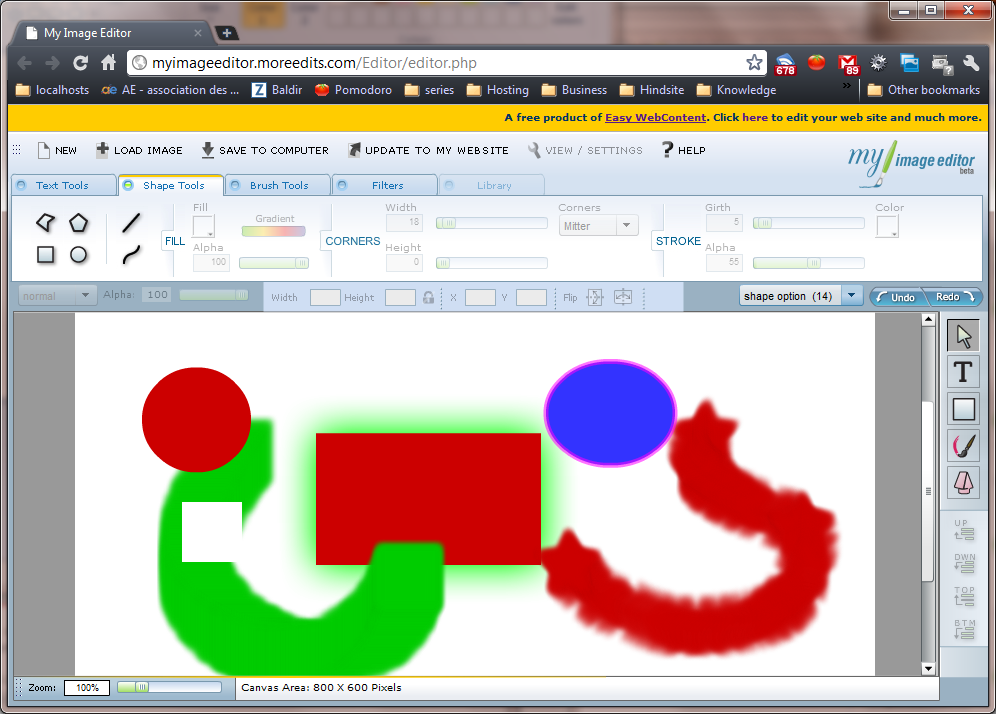
\includegraphics[width=.80\textwidth]{img/my_image_editor.png}
\caption{My Image Editor}
\label{figure:ewc-image_editor}
\end{figure}

I had first to "enter" head-first into the code written by the 3 previous interns. I was not very familiar with the Actionscript 3 programmation language but it is very similar to Java which I know better. One of the bigger difficulties was to deal with a main class file of more than 6000 lines of code. I could not refactor\footnote{Refactoring is a disciplined technique for restructuring an existing body of code, altering its internal structure without changing its external behavior (Martin Fowler \url{http://www.refactoring.com/)}} this piece of code because it would need too much time. 

I had to secure the swf file\footnote{file generated by Flash that can be embedded in a web page} by  using some URL rewrite technique and server side processing with PHP. Basically a PHP file with the .swf extension is used to import the file stream of the flash file. I added server directives to make .swf files interpreted as PHP scripts instead of directly downloaded. The PHP script require a session which is created by the script which want to embed the flash object. If the session is not found (which means that someone want to download the original .swf file by from its url it will return an error page instead of the file).

\lstset{language=PHP}
\begin{lstlisting}[label=swf-secure,caption=PHP script disguised into a swf file to avoid direct download]
	//retrieve the session
	session_start();
	//Test if the variable"flash" is directly access to prevent direct access by typing
	//the url of the swf file in the browser
	if(isset($_SESSION["flash"]))
	{
		$referrer = $_SERVER["HTTP_REFERER"];
		$referrer = parse_url($referrer);

		//Test if the domain are the same to prevent the access for others domains
		if($referrer["host"] != $_SESSION["flash"])
		{
			echo "Permission denied.";
			exit();
		}

	}
	else
	{
		echo "Permission denied.";
		exit();
	}
	//Destroy the session
	unset($_SESSION["flash"]);
	//Get the SWF if the test	
	header ("Cache-Control: no-cache, must-revalidate");
	header("Content-Type: application/x-shockwave-flash");
	readfile($_SERVER["DOCUMENT_ROOT"].'/Editor/01_Template.swf');
\end{lstlisting}
%$


I also had to add a preloader(cf. \ref{figure:ewc-image_preloader} p.\pageref{figure:ewc-image_preloader}) to the page embedding My Image Editor. The aim of this manipulation is to show a loading animation instead of a blank page while witing that the complete editor and its assets are fully loaded. In order to achieve this task the Image Editor had to communicate its status to the embedding page through a library called ExternalInterface. 

\begin{figure}[!h]
\centering
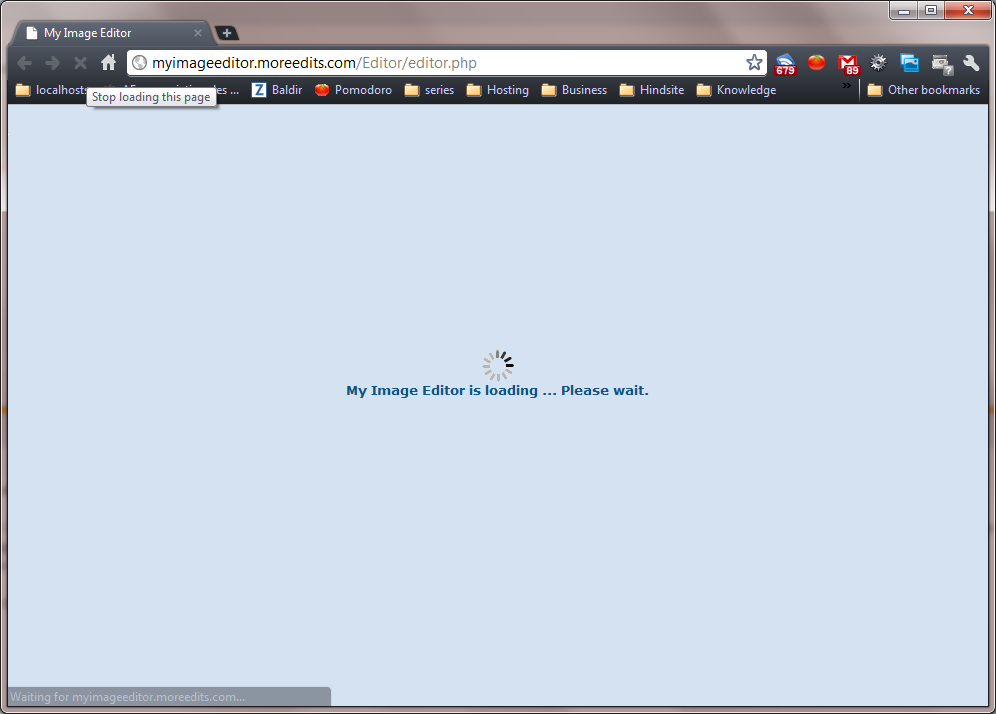
\includegraphics[width=.80\textwidth]{img/myimage_preloader.png}
\caption{My Image Editor preloader}
\label{figure:ewc-image_preloader}
\end{figure}

During the next weeks I was assigned more complex tasks which I will talk in the following chapters.

\section{Agenda of the Internship}

The table \ref{tableau:agenda} presents the different task I was assigned during my internship.

\begin{table}[!h]
	\caption{\label{tableau:agenda}Internship Agenda}
	\begin{tabular}{ | l | p{12cm} | }
		\hline
		 & Tasks\\
		\hline
		Week 1	&	Population of content for Sencore's website\\	\hline
		Week 2	&	Development of Sencore's Website. Read documentation of the different projects of Hindsite Interactive. Get comfortable with the main project Easy Web content.\\	\hline
		Week 3 to 4	&	Work on Easy Web Content's Image Editor. Issues fixes.\\	\hline
		Week 5 to 7	&	Work both on the Image Editor and the specifications of the new Easy Web Content's Site Builder. Implementation of Performance Improvement tools.\\	\hline
		Week 8 to 12	&	Brainstorming and resarches about the Site builder features. Study the conpetitors. MVC Framework development.\\	\hline
		Week 12 to 16	&	Application of web design on the tools of the Site builder. Database development, drag and drop. User registration. Database automated scripts.	\\	\hline
		Week 17	to 18&	Work on Site Builder's widget features. Implementation of Video player feature on Sencore project. Work on secured payment form on A2LA project. Begin to communicate with clients.\\	\hline
		Week 19	to 22 &	Work on a mailling form for the client Advanced Centrifugals coupled with a backend. Bug correction on Sencore and Sentara projects. Work on the Site Builder in parallel\\	\hline
		Week 23	to 24&	Work on Pylon Project\\	\hline
	\end{tabular}
\end{table}

\section{Methodological aspect}

Hindsite Interactive possess more than 10 year in web design and development. During these years 
some methodological standards has been established.

\subsection{Specification of the needs}
This step is a discussion with the customer to understand his expectations
and needs as well as establish a quote for the job and determine the duration
of the development.
This phase will for instance estimate the number of pages, the design work (if
the users wants Flash animations, unique fonts, a new logo, etc.), the degree
of administration possibilities (static HTML, partially manageable, or a full
CMS).

This step is supervised by Mr. Taei, who consults designers or developers to
get an accurate idea of the cost, time and possibilities.

\subsection{Presentation of one or many prototype}
The next step consists of a presentation of a static design of the future web
site layout. Many different designs can be showed to the client to allow him to
choose the one that better fits his expectations.
The design is done by the design team, most of the time by Mr. Kheradmand.

\subsection{Conversion of the design to HTML and CSS}
This phase is made up of the slicing of design elements (backgrounds,
images, titles, etc.) to images and of the conversion to a static design into the
HTML/CSS website. All the text content is static at this phase.

%This step is usually affected to Mrs. Hang Le, but I happen to give a hand for
some CSS tricks or JavaScript animations/modules.

- The development, add the Content Management System.
During the next phase, the dynamic pages are written, all the pages which
content need to be editable by the client are integrated in the administration
area. This is the phase that most concerns me and other coworkers of the
development team.

- Presentation and Validation
The website (at this moment hosted on Hindsite’s servers) is presented to the
client for validation. We give him an access to the administration area to test
the different functionalities and we provide him explanation of how to use it if
necessary.

- Deployment
When the website is approved, we move on to the deployment on either client
hosting server or our server with the definitive DNS redirection. We also use a
clean database from all the tests.

\section{Technical aspect}

%ActionScript 3 is a programming language based on the ECMAScript
%standard and is mainly used for website development or software based on
%Adobe Flash Player. AS3 allows communication of the application and the
%server or a database. Powered by Macromedia and then Adobe, ActionScript
%actually allows to developer Rich Internet Applications and online games.
%
%PHP is an open source script languages, used to produce dynamic web pages
%through an HTTP server. PHP is an imperative language and supports Object
%Oriented programming since the version 5. For the Easy Web Content
%modules we use PHP5 but for website development, it can depend of the
%version already in place.
%
%JavaScript is a script language typically used to enable access to
%computational objects within a host environment. It is used as a client-side
%language for the development of dynamic Internet websites.
%
%WEINZAEPFEL Pierre
%
%jQuery
%A fast, concise, library that simplifies how to traverse HTML documents,
%handle events, perform animations, and add AJAX.
%
%Smarty is a library that allows the creation of HTML templates that are imported and
%used in PHP scripts to ease the process of web page design.
%
%One of Smartys primary design goals is to facilitate the separation of application
%code from presentation.
%Typically, the application template containing the design is separated from the PHP
%code.
%
%I used Smarty as a template engine to generate the templates pages of the
%administration page of the add-on.

\section{Tools}

%a. Astah Community
%
%I have been using Astah Community -previously called Jude Community- to
%design my Use Case, Class, Sequence, etc. diagrams.
%This software takes place at the beginning of the development cycle, in
%analyze and conception phases.
%
%b. FlashDevelop
%
%FlashDevelop is a free and open source code editor for Action Script 2.0 and
%3.0.
%It has a development environment visually similar to that of Eclipse. It has a
%collapsible file explorer that makes projects easier to navigate.
%In my opinion FlashDevelop is more user-friendly and easy to use than the
%Action Script editor integrated into Adobe Flash Professional. Flash Develop is
%only used to edit the code, there is no timeline visualization, image browser or
%object (buttons, movie clips) library.
%FlashDevelop is linked to Flash Professional so that I can directly test
%changes in Flash Pro.
%
%WEINZAEPFEL Pierre
%
%This software was used in the implantation (code writing) step in the software
%development cycle.
%
%c. Adobe Flash CS4
%
%It is a multimedia platform developed by Adobe that enables to create
%interactive content for web pages like animations, advertisements, games, etc.
%
%d. Dreamweaver CS4
%It’s a website editor also by Adobe that offers much functionality to improve
%development. It supports a lot of web technologies (XHTML, PHP, CSS, and
%JavaScript). It is also possible to use subversion directly inside the navigation
%panel.
%
%e. Vizzy
%
%Vizzy is a free software for Flash development, this tool allows seeing all
%traces (display a result to the output window) and debugging content of Flash
%files (.swf)